%\chapter{F\'isica y Medici\'on}\label{ch:fisicamedicion}
%

\epigraph{All science is either physics or stamp collection.}{\textit{Ernest Rutherford}}

?`Qu\'e tanto sabemos realmente de nuestro Universo? ?`C\'omo podemos asegurarnos de que lo que descubramos sea cierto en otro momento en la historia, as\'i como en otras condiciones f\'isicas? ?`Es realmente necesario conocer a profundidad la historia de la tecnolog\'ia y conocimiento que tenemos hoy en d\'ia, o basta con concertrarnos en futuros experimentos? ?`Se nace uno siendo cient\'ifico, o se cultiva \'este tipo de pensamiento?

\section{Introducci\'on}\label{sec:intro1}

En el Cap\'itulo 1 de su libro de texto, se introducen un poco las \'areas en las cuales est\'a descompuesta el \'area de la F\'isica; quiz\'a podemos ahondar un poco m\'as en el tema. Si bien la F\'isica estudia todo fen\'omeno que podemos encontrar en la naturaleza, sus or\'igenes datan \'unicamente en aquellos fen\'omenos que se pod\'ian observar directamente. ?`C\'omo es posible, entonces, que podamos generar (y generalizar) ideas que sean aplicables para fen\'omenos naturales que a\'un no podamos observar o inclusive que nunca podremos observar directamente?

Si bien \'esta duda no es \'unica para la F\'isica, es una que ha persistido a lo largo de su historia. En efecto, la importancia de la F\'isica radica en su objetivo principal de estudiar los principios b\'asicos de la naturaleza y expresar a \'estos en el lenguaje de la \textit{matem\'atica}. El prop\'osito de \'esto es simple: poder predecir y por lo tanto, manipular, a la naturaleza para nuestra ventaja, adem\'as de la belleza intr\'insica que \'esto posee.

Si bien \'esto \'ultimo suena algo l\'ugubre, no lo es: teniendo \textbf{modelos} de fen\'omenos f\'isicos podremos, por ejemplo, estudiar errores pasados en la construcci\'on de puentes\footnote{Destrucci\'on del Puente de Tacoma Narrows en 1940, WA, EE.UU. \href{https://goo.gl/NyR1jp}{https://goo.gl/NyR1jp}} y as\'i evitar posibles p\'erdidas humanas (sin mencionar las materiales). Es de notar, entonces, que las caracter\'isticas que deseamos en nuestros modelos es que se utilizen la menor cantidad de conceptos, ecuaciones y suposiciones y que sean lo m\'as general posibles.

Respecto a \'este \'ultimo punto, debemos de hacer \'enfasis en lo siguiente: los modelos que generemos \textbf{\emph{NO}} son sustituto para el problema original. En efecto, s\'olo son simplificaciones de \'este para as\'i poder llegar a una soluci\'ion de una manera simple. \'Esto no quiere decir que las soluciones a las que lleguemos sean err\'oneas, sino que simplemente no ser\'an \emph{absolutamente precisas}, s\'olo hasta cierta tolerancia. Otro punto a hacer \'enfasis en la F\'isica (y Ciencias Naturales en general), es que s\'olo porque una teor\'ia tenga evidencia a su favor no quiere decir que sea infalible. Al contrario, se busca siempre encontrar posibles experimentos donde las teor\'ias fallen para as\'i descartar aquellas que no sean siempre generales. 

Cuando las predicciones hechas por los modelos son simplemente err\'oneos, entonces sabremos que las suposiciones no se est\'an cumpliendo o bien que la teor\'ia/modelo no es el adecuado. Es de recalcar, entonces, que si las suposiciones b\'asicas de nuestros modelos no se cumplen, entonces es il\'ogico esperar que los modelos se cumplan\footnote{Sobre la crisis econ\'omica del 2008: \href{https://goo.gl/jLb52T}{https://goo.gl/jLb52T}}.

Es as\'i como han nacido algunas de las distintas \'areas en las que se descompone la F\'isica. A grandes rasgos, \'estas son:

\begin{description}
    \item [Mec\'anica cl\'asica] Desarrollada principalmente por Isaac Newton (1642-1727). Es el \'area de la F\'isica que estudia el movimiento de los objetos "grandes" ($\gg\SI{e-9}{\meter}$) y que viajen a velocidades mucho menores del de la luz en el vac\'io ($\ll\SI{299792458}{\meter/\second}$). V\'ease Figura \ref{fig:mec_clasica} y Figura \ref{fig:newt_v_einst}.
    
\begin{figure}
\centering
\begin{subfigure}{.45\textwidth}
  \centering
  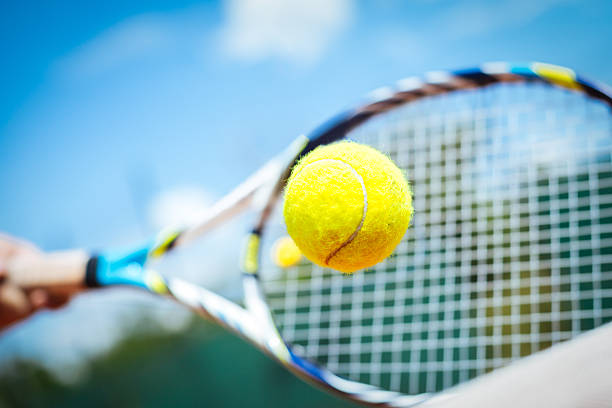
\includegraphics[width=.95\textwidth]{lecture1/tennis.jpg}
  \caption{La trayectoria de una pelota de tennis puede ser descrita sin tener que recurrir a teor\'ias avanzadas}
  \label{fig:sub_tennis}
\end{subfigure}%
\hfill
\begin{subfigure}{.45\textwidth}
  \centering
  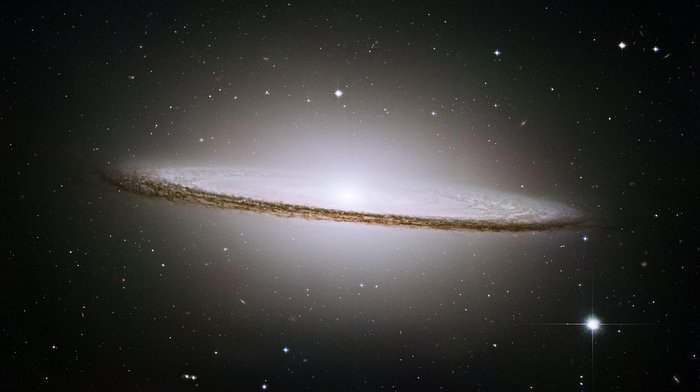
\includegraphics[width=.95\textwidth]{lecture1/sombrero.jpg}
  \caption{La Galaxia Sombrero, o Messier 104 (M104). Cr\'editos NASA/ESA y el Hubble Heritage Team}
  \label{fig:sub_galaxia}
\end{subfigure}
\caption{Dos objetos, si bien de tama\~nos abismalmente distintos, que pueden ser descritos utilizando las ecuaciones de la Mec\'anica Cl\'asica.}
\label{fig:mec_clasica}
\end{figure}
    
    \item [Relatividad] Teor\'ia generada por Albert Einstein (1879-1955) que puede describir todo objeto grande ($\gg\SI{e-9}{\meter}$) que viaje a cualquier velocidad\cite{einstein} (Mec\'anica Relativista). Sin embargo, impone un l\'imite superior a la velocidad: la de la luz ($c=\SI{299792458}{\meter/\second}$). V\'ease las Figuras \ref{fig:newt_v_einst} y  \ref{fig:aceleradores}.
    
\begin{figure}
\centering
\begin{subfigure}{.45\textwidth}
  \centering
  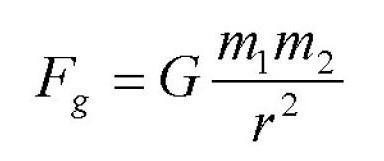
\includegraphics[width=\textwidth]{lecture1/newtongrav.jpg}
  \caption{La Ley de Gravitaci\'on Universal de Newton, la cual podremos llegar a ver m\'as adelante en este curso.}
  \label{fig:sub_newton}
\end{subfigure}%
\hfill
\begin{subfigure}{.45\textwidth}
  \centering
  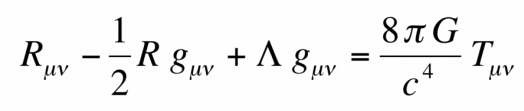
\includegraphics[width=\textwidth]{lecture1/einsteinfieldeq.jpg}
  \caption{Las Ecuaciones de Campo de Einstein.}
  \label{fig:sub_einstein}
\end{subfigure}
\caption{Dos ecuaciones que describen la interacci\'on gravitacional entre dos objetos, como se muestra en la portada de \'estas notas de curso. ?`Cu\'al escoger\'ia usted para modelar correctamente la trayectoria de un sat\'elite de GPS? ?`Por qu\'e?}
\label{fig:newt_v_einst}
\end{figure}
    
    \item [Termodin\'amica] \'Area de la F\'isica desarrollada con el fin de incrementar la eficiencia de las m\'aquinas de vapor por el franc\'es Nicolas L\'eonard Sadi Carnot (1796-1832). Las \'areas de inter\'es son el calor, el trabajo, la temperatura y el comportamiento estad\'istico de los sistemas con gran n\'umero de part\'iculas (Mec\'anica Estad\'istica).
    \item [Electromagnetismo] Teor\'ia generada por James Clerk Maxwell (1831-1879) al unir las dos \'areas que previamente se cre\'ian que eran separadas: electricidad y magnetismo. V\'ease la Figura \ref{fig:aceleradores}.
    
\begin{figure}
\centering
\begin{subfigure}{.45\textwidth}
  \centering
  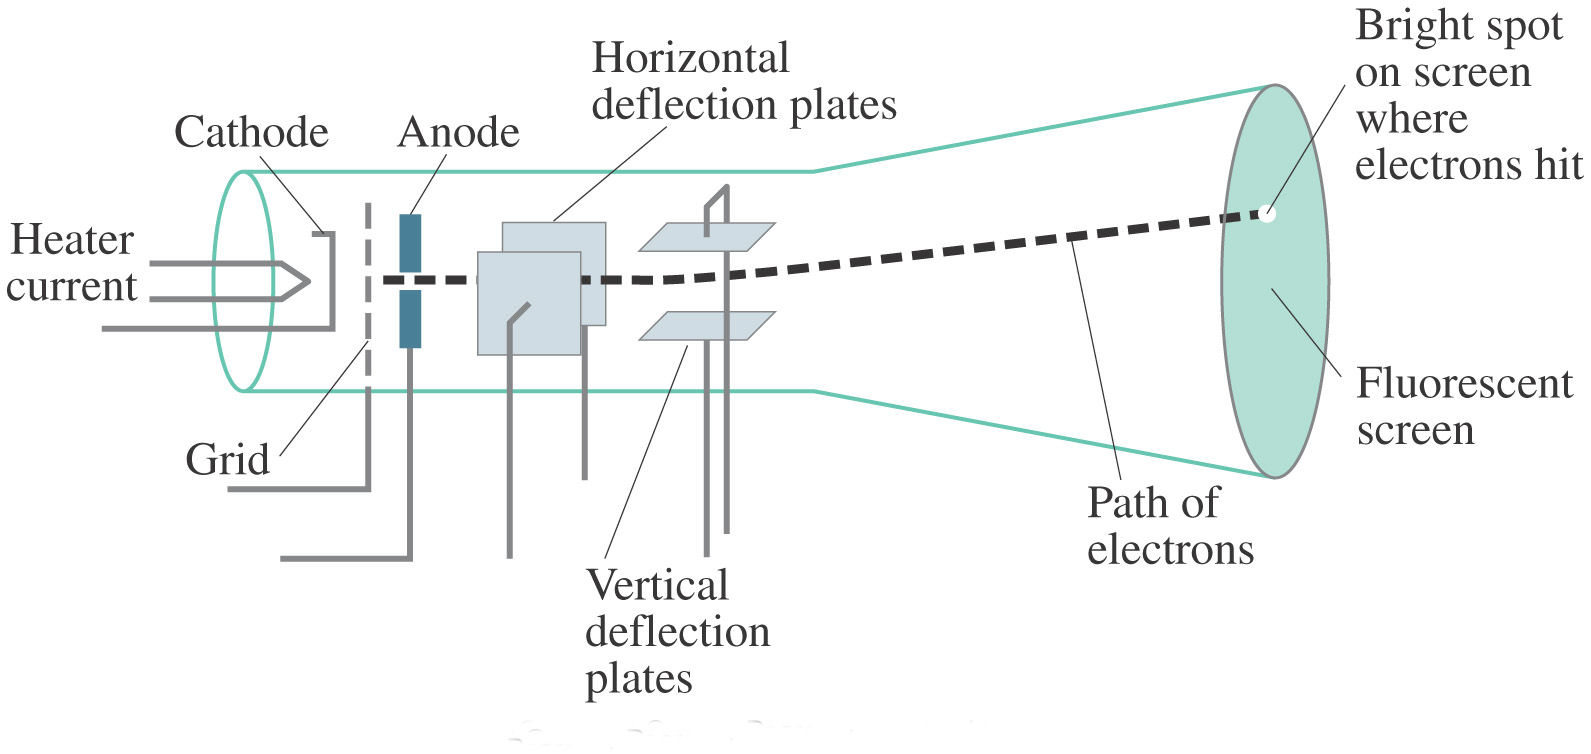
\includegraphics[width=\textwidth]{lecture1/Cathode-Ray-Tube-Diagram.jpg}
  \caption{Los primeros televisores usaban un peque\~no acelerador de part\'iculas llamado tubo de rayos cat\'odicos.}
  \label{fig:sub_cathode}
\end{subfigure}%
\hfill
\begin{subfigure}{.45\textwidth}
  \centering
  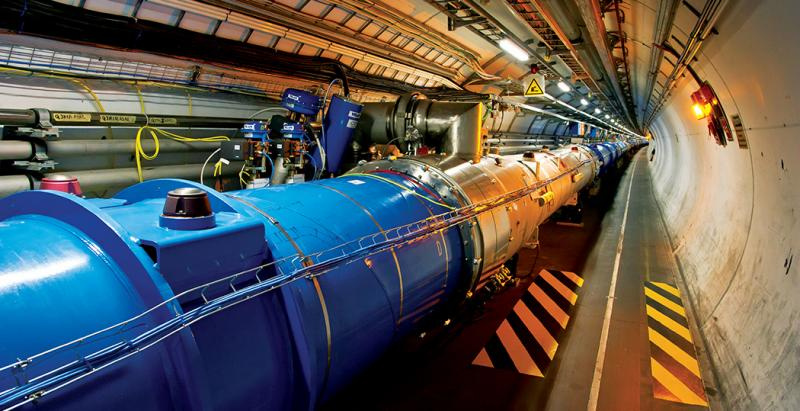
\includegraphics[width=\textwidth]{lecture1/lhc_long.jpg}
  \caption{El Gran Colisionador de Hadrones (LHC) en Ginebra, Suiza.}
  \label{fig:sub_lhc}
\end{subfigure}
\caption{Si bien la teor\'ia de Maxwell no ha cambiado, la tecnolog\'ia si lo ha hecho y se \href{https://horizon-magazine.eu/article/physicists-accelerate-plans-new-large-hadron-collider-three-times-big_en.html}{planea en seguir avanzando}.}
\label{fig:aceleradores}
\end{figure}

    \item [\'Optica] \'Area de la F\'isica que se encarga del estudio de la luz y su interacci\'on con distintos materiales.
    \item [Mec\'anica cu\'antica] Teor\'ia generada de manera separada por varios cient\'ificos a partir del siglo XVII. Es el \'area de la F\'isica que estudia el movimiento de los objetos "peque\~nos" ($\ll\SI{e-9}{\meter}$)\footnote{El por qu\'e se busca otra tecnolog\'ia para hacer transistores menores a \SI{7}{\nano\meter}, \href{https://goo.gl/WRqFmD}{https://goo.gl/WRqFmD}. } y que viajen a velocidades mucho menores del de la luz en el vac\'io  ($\ll\SI{299792458}{\meter/\second}$). Si bien existen experimentos mentales \href{http://www.fisicafundamental.net/misterios/gato.html}{famosos}, \'esta \'area tiende a ser categ\'oricamente   \href{http://cosmology.com/ConsciousTime107.html}{malinterpretada}.
\end{description}

Si bien \'esta lista no es exhaustiva, cubre la mayor\'ia de las \'areas en las cuales se descompone el \'area de la F\'isica actual. Recu\'erdese que una teor\'ia m\'as general no siempre reemplazar\'a a otra m\'as simple: en efecto, para calcular la trayectoria de un proyectil, utilizaremos las ecuaciones de la Mec\'anica Cl\'asica y no las de Einstein, ya que \'esto implicar\'ia solamente desperdiciar esfuerzos y recursos. Sin embargo, no es de sorprenderse de que se descarten algunas de estas teor\'ias en el futuro por otras teor\'ias m\'as generales.

%
\section{Est\'andares de Longitud, Masa y Tiempo}\label{sec:estandares1}
%

Debido a que queremos expresar a las teor\'ias y leyes de la F\'isica usando el lenguaje de las matem\'aticas, ciertas cantidades f\'isicas aparecen de vez en cuando. \'Estas se dividen en \emph{cantidades fundamentales} y \emph{cantidades deducidas}, donde las \'ultimas pueden ser expresadas como una combinaci\'on de las primeras. En la Mec\'anica, las tres cantidades fundamentales son \textbf{longitud}, \textbf{masa} y \textbf{tiempo}.

Si bien queremos \emph{reproducir} los resultados obtenidos previamente por nosotros o otro grupo investigativo, o viceversa, debemos de definir cierto \emph{est\'andar}. En 1960, se cre\'o el \textbf{Sistema Internacional} o \textbf{SI} (Syst\`eme International) en el cual se definieron las unidades de longitud, masa y tiempo son el \textbf{metro} (\SI{}{\meter}), el \textbf{kilogramo} (\SI{}{\kilogram}) y el \textbf{segundo} (\SI{}{\second}), respectivamente. Otros est\'andares de SI establecidos fueron las de la temperatura (el \emph{kelvin} \SI{}{\kelvin}), corriente el\'ectrica (el \emph{ampere} \SI{}{\ampere}), la intensidad luminosa (la \emph{candela} \SI{}{\candela}) y la cantidad de sustancia (el \emph{mol} \SI{}{\mole}).

Para las cantidades fundamentales de la Mec\'anica, se han acoplado los siguientes est\'andares:

\begin{description}
    \item [Longitud] En Octubre de 1983, se [re]defini\'o el metro \SI{}{\meter} como \textbf{la distancia recorrida por la luz en el vac\'io durante un tiempo de \SI{1/299792458}{\second}}.
    \item [Masa] Se estableci\'o el kilogramo \SI{}{\kilogram} en 1887 como \textbf{la masa de un cilindro de aleaci\'on platino-iridio espec\'ifico que se conserva en la Oficina Internacional de Pesos y Medidas (BIPM) en S\`evres, Francia}.
    \item [Tiempo] En 1967, se [re]defini\'o al segundo \SI{}{\second} utilizando un \emph{reloj at\'omico} de la siguiente manera: \textbf{\SI{9192631770}{} veces el per\'iodo de vibraci\'on de la radiaci\'on del \'atomo de cesio 133}.
\end{description}

Si bien \'estas definiciones parecen ser algo rebuscadas, al parecer lo son para los nuevos est\'andares internacionales. En efecto, se \href{https://www.bipm.org/utils/common/pdf/SI-statement.pdf}{redefinir\'an todas las unidades del SI en Noviembre del presente a\~no}. Se espera que \'estas redefiniciones entren en vigor el 20 de Mayo de 2019. En res\'umen, las redefiniciones del kilogramo, ampere, kelvin y mol ser\'an basadas en t\'erminos de siete constantes f\'isicas, de la misma manera en que el metro est\'a basado en la velocidad de la luz. A ra\'iz de \'esto, las unidades de SI no tendr\'an que ser modificadas conforme las mediciones e instrumentaci\'on avanzen en el futuro. 

En las Tablas \ref{table:distancias1}, \ref{table:masas1} y \ref{table:tiempos1}, se presentan algunas medidas de distintos rangos de longitud, masa e intervalos de tiempo. Tener a la mano \'este tipo de valores o tablas es importante ya que nos servir\'a para poder discernir si los resultados que obtenemos est\'an en un rango aceptable, o bien si existe la posibilidad de que se cometi\'o un error en el camino.

\begin{table}[ht]
\caption{Valores aproximados de algunas longitudes medidas}
\begin{tabular}{l r}
\toprule
           & \textbf{Longitud (\SI{}{\meter})} \\
\midrule
Di\'ametro del Universo Observable & $8.8\times10^{26}$\\
Distancia de la Tierra a la galaxia m\'as cercana (Andr\'omeda) & $2\times10^{22}$\\
Distancia del Sol a la estrella m\'as cercana (Pr\'oxima Centauri)  &  $4\times10^{16}$  \\
Radio orbital promedio de la Tierra alrededor del Sol &  $1.50\times10^{11}$ \\
Radio del agujero negro Sagitario $A^*$ en el centro de la V\'ia L\'actea & $1.2\times10^{10}$\\
Radio medio de la Tierra & $6.37\times10^{6}$\\
Altitud t\'ipica s.n.m. de un sat\'elite que orbita la Tierra & $2\times 10^5$\\
Longitud de una mosca & $5\times10^{-3}$\\
Tama\~no de las c\'elulas de la mayor\'ia de los seres vivos & $\sim10^{-5}$ \\
Di\'ametro de un \'atomo de hidr\'ogeno & $\sim10^{-10}$\\
Di\'ametro de un prot\'on & $\sim10^{-15}$\\
\bottomrule
\end{tabular}
\label{table:distancias1}
\end{table}

\begin{table}[t]
\caption{Masas aproximadas de varios objetos}
\begin{tabular}{l r}
\toprule
           & \textbf{Masa (\SI{}{\kilogram})} \\
\midrule
Universo Observable & $\sim10^{52}$\\
V\'ia L\'actea & $\sim10^{42}$\\
Gargantua (\emph{Interstellar})  &  $2\times10^{38}$  \\
Sagitario $A^*$ &  $4.31\times10^{36}$ \\
Sol & $1.99\times10^{30}$\\
Tierra & $5.98\times10^{24}$\\
Humano & $\sim 10^2$\\
Mosquito & $\sim10^{-5}$\\
Bacteria & $\sim10^{-15}$ \\
\'Atomo de hidr\'ogeno & $1.67\times10^{-27}$\\
Electr\'on & $9.11\times10^{-31}$\\
\bottomrule
\end{tabular}
\label{table:masas1}
\end{table}


\begin{table}[t]
\caption{Valores aproximados de algunos intervalos de tiempo}
\begin{tabular}{l r}
\toprule
           & \textbf{Intervalo de Tiempo (\SI{}{\second})} \\
\midrule
Edad del Universo & $4.35\times10^{17}$\\
Edad de la Tierra & $1.43\times10^{17}$\\
Un a\~no  &  $3.2\times10^{7}$  \\
Un d\'ia (revoluci\'on de la Tierra sobre su eje) &  $8.6\times10^{4}$ \\
Un per\'iodo de clase & $2.7\times10^{3}$\\
Latido normal & $8\times10^{-1}$\\
Tiempo que le toma a un prot\'on dar una vuelta al LHC & $\sim 10^{-4}$\\
Intervalo de tiempo para que la luz cruze un prot\'on & $\sim10^{-24}$\\
\bottomrule
\end{tabular}
\label{table:tiempos1}
\end{table}

Adem\'as de \'estos valores normales, existen prefijos para denotar las potencias en la notaci\'on cient\'ifica y evitar potencias muy grandes o muy peque\~nas, como lo son nano (\si{\nano}), micro (\si{\micro}), centi (\si{\centi}), kilo (\si{\kilo}), mega (\si{\mega}), giga (\si{\giga}), entre otros. \'Estos no se les quedar\'an memoriz\'andose \'esta tabla, sino con la pr\'actica, as\'i como su uso diario. Para una mejor referencia, vea la Tabla 1.4 de su libro de texto.


\section{An\'alisis Dimensional}\label{sec:analisisdim1}

En la F\'isica, llamamos a la \emph{dimensi\'on} a la naturaleza f\'isica de una cantidad. Es decir, no importa si expresamos las medidas de un objeto en metros, pies o pulgadas, siempre seguimos hablando de una distancia. Lo mismo sucede para las otras dos cantidades fundamentales de masa y tiempo. 

Se utilizar\'an, entonces, a los s\'imbolos \si{\length}, \si{\mass} y \si{\time} para denotar a las dimensiones de longitud, masa y tiempo, respectivamente. Adem\'as, utilizaremos los corchetes $[\cdot]$ para denotar que estamos analizando las dimensiones de una cantidad f\'isica. Apliquemos \'esto a un ejemplo:

\begin{ejemplo}
Encuentre las dimensiones del \'area de un cuadrado de lado $a$.
\label{ej:area}
\end{ejemplo}

\begin{solution*}Aplicamos nuestro operador $[\cdot]$ a la f\'ormula o ecuaci\'on del \'area $A$ de un cuadrado:

\[ [A] = [a^2] = [a]\cdot[a] = \si{\length}\cdot\si{\length} = \si{\length}^{2} \]\hfill$\square$

\end{solution*}

Por lo tanto, el \textbf{an\'alisis dimensional} puede ser utilizado para verificar que una ecuaci\'on est\'e escrita de manera correcta, especialmente cuando veamos t\'erminos en nuestras ecuaciones que tengan potencias distintas a uno. Asimismo, nos ser\'a \'util para verificar que nuestro resultado final sea correcto, si es que existe alguna duda al respecto.

En res\'umen, el poder del an\'alisis dimensional yace en que las \textbf{dimensiones pueden ser tratadas como cantidades algebraicas}, como hemos hecho en el Ejemplo \ref{ej:area}. Dicho de otra manera, podemos sumar o restar cantidades \'unicamente si tienen las mismas dimensiones y una ecuaci\'on tiene sentido solamente si ambos lados de \'esta tienen las mismas dimensiones. 

\begin{table}[t]
\caption{Unidades y unidades de distintas cantidades deducidas}
\begin{tabular}{l ccccc}
\toprule
Cantidad  & \textbf{Vol\'umen ($V$)} & \textbf{Rapidez ($v$)} & \textbf{Aceleraci\'on ($a$)} & \textbf{Fuerza ($F$)}\\
\midrule
Dimensiones & $\si{\length}^{3}$ & $\si{\length}/\si{\time}$ & $\si{\length}/\si{\time}^{2}$ & $\si{\mass}\cdot\si{\length}/\si{\time}^{2}$\\
Unidades SI & $\si{\meter}^{3}$ & $\si{\meter}/\si{\second}$ & $\si{\meter}/\si{\second}^{2}$ & $\si{\kilogram}\cdot\si{\meter}/\si{\second}^{2}$\\
\bottomrule
\end{tabular}
\label{table:dimensiones}
\end{table}

Utilizando la Tabla \ref{table:dimensiones}, proseguimos a resolver ejemplos m\'as complejos:

\begin{ejemplo}
\textcolor{red}{\textbf{\hl{W}}} En la Figura \ref{fig:sub_newton} vemos la Ley de Gravitaci\'on de Newton, la cual nos permite calcular la fuerza gravitatoria que ejercen dos cuerpos entre s\'i, i.e.:

\[ F_{g} = G \frac{m_{1}m_{2}}{r^{2}}\]

donde $F_{g}$ es la fuerza gravitatoria, $G$ es la constante de gravitaci\'on universal de Newton, $m_{1}$ y $m_{2}$ son las masas de los dos objetos y $r$ es la distancia entre \'estos. Encuentre las dimensiones de $G$.
\label{ej:newton}
\end{ejemplo}

\begin{solution*}Aplicamos nuestro operador $[\cdot]$ a ambos lados de la ecuaci\'on y utilizando la Tabla \ref{table:dimensiones}:

\begin{align*}
    [F_{g}] &= [G \frac{m_{1}m_{2}}{r^{2}}] \\
    \implies \si{\mass}\frac{\si{\length}}{\si{\time}^{2}} &= [G] \frac{\si{\mass}^{2}}{\si{\length}^{2}}\\
    \implies [G] &= \cancel{\si{\mass}}\frac{\si{\length}}{\si{\time}^{2}} \frac{\si{\length}^{2}}{\cancel{\si{\mass}^{2}}}\\
    \therefore [G] &= \frac{\si{\length}^{3}}{\si{\mass\time^{2}}}
\end{align*} \hfill$\square$

%\si[per-mode = fraction]{\cancel\kilogram\metre\per\cancel\kilogram\per\second}

\end{solution*}

Es de notar que el an\'alisis dimensional \textbf{\emph{NO}} nos dar\'a los valores num\'ericos de las constantes en las ecuaciones, solamente sus dimensiones. Dichos valores de las constantes aparecen \'unicamente a trav\'es de la experimentaci\'on, algo que veremos en los laboratorios m\'as adelante.

\begin{ejercicio}
Una cantidad deducida es la \textbf{densidad} de un objeto de masa $m$ que ocupa un vol\'umen $V$. \'Esta se denota por $\rho$ y se calcula de la siguiente manera:

\begin{equation}
    \rho = m/V
\end{equation}

Encuentre las dimensiones en el SI para la densidad $\rho$.
\end{ejercicio}

\begin{ejercicio}
Nos dicen que la aceleraci\'on $a$ de una part\'icula de massa $m$ que se mueve a una rapidez constante $v$ en una trayectoria circular de radio $r$ es proporcional a alguna potencia de $r$ (digamos $r^{\alpha}$), a alguna potencia de $v$ (digamos $v^{\beta}$) y a alguna potencia de $m$ (digamos $m^{\gamma}$). Encuentre los valores de las potencias.
\end{ejercicio}

\section{Conversi\'on de Unidades}\label{sec:conversion1}

No todos los pa\'ises o instituciones alrededor del mundo utilizan las mismas unidades, a veces debemos de cambiar de un sistema (como el SI) a otro (como el de Unidades de medida de Estados Unidos, \href{https://es.wikipedia.org/wiki/Unidades_tradicionales_de_Estados_Unidos}{USCS}). A menos que querramos aparecer en vergonzosas listas\footnote{V\'ease, por ejemplo: \url{https://goo.gl/z35nY7}}, por no mencionar los riesgos a la vida humana. Por lo tanto, es de vital importancia que puedan realizar la conversi\'on de unidades de manera correcta. Hist\'oricamente, donde m\'as se ha visto \'esto es en su curso de Qu\'imica, por lo que espero que \'esta no sea la primera vez que vean \'este tipo de conversiones.

La conversi\'on de unidades puede ser tanto entre sistemas (SI a USCS, e.g., de kil\'ometros a millas), o bien dentro de un sistema (e.g., de metros a kil\'ometros). Algunos ejemplos de \'este tipo de conversiones entre sistemas son (pero no dude de revisar el Ap\'endice A de su libro de texto para la lista completa):

\begin{equation*}
\begin{aligned}[c]
\SI{1}{\milla}&=\SI{1609}{\meter} = \SI{1.609}{\kilo\meter}\\
\SI{1}{\meter}&=\SI{39.37}{\inch} = \SI{3.281}{\pie}
\end{aligned}
\hspace{10mm}
\begin{aligned}[c]
\SI{1}{\pie}&=\SI{0.3048}{\meter} = \SI{30.48}{\centi\meter}\\
\SI{1}{\inch} &= \SI{0.0254}{\meter} = \SI{2.54}{\centi\meter} 
\end{aligned}
\end{equation*}

Siguiendo la misma l\'inea del an\'alisis dimensional visto en la Secci\'on \ref{sec:analisisdim1}, las unidades entonces tambi\'en pueden ser tratadas como cantidades algebraicas. Es decir, podemos sumarlas siempre que sumemos metros con metros, por ejemplo, y podemos cancelarlas si se dividen entre s\'i y se trate de la misma unidad.

\begin{ejemplo}
Por alguna raz\'on, usted decidi\'o comprarle un veh\'iculo a una su conocida. Sin embargo, el indicador de velocidad muestra \'unicamente la rapidez en millas por hora (\si{\milla/\hour}). Si el l\'imite de velocidad en la carretera donde est\'a manejando es de \SI{70}{\kilo\meter/\hour} y el indicador dice que usted viaja a \SI{60}{\milla/\hour}, ?`rebas\'o usted el l\'imite de velocidad?
\end{ejemplo}

\begin{solution*}
Usando ya sea el Ap\'endice A o la peque\~na lista que les proporcion\'e anteriormente, podemos convertir las millas a kil\'ometros para as\'i convertir la rapidez en kil\'ometros por hora. Multiplicamos, entonces a la rapidez dada por un neutro multiplicativo, i.e.:

\[ \SI{60}{\milla/\hour} = 60 \frac{\cancel{\si{\milla}}}{\si{\hour}} \left(\frac{\SI{1.609}{\kilo\meter}}{1\cancel{\si{\milla}}}\right) = \SI{96.54}{\kilo\meter/\hour} \]

Es decir, EMETRA le dar\'a una jugosa multa (asumiendo que una c\'amara o polic\'ia lo haya capturado en el acto).\hfill $\square$
\end{solution*}

\begin{ejercicio}
La estrella m\'as cercana al Sol, Pr\'oxima Centauri, se encuentra a aproximadamente \SI{4e13}{\kilo\meter} de distancia. Se define a un a\~no luz (\si{\aluz}) como la distancia que recorre la luz en un a\~no. Convierta \'esta distancia de \si{\kilo\meter} a \si{\aluz}
\end{ejercicio}


\section{Estimaciones y C\'alculos de Orden de Magnitud}\label{sec:ordenmagn1}

En \href{https://www.quora.com/If-you-were-at-a-Google-interview-how-would-you-answer-How-many-views-does-YouTube-have-per-day}{las afamadas entrevistas de Google}\footnote{\'Este tipo de problemas se conocen como Problemas de Fermi en homenaje al famoso f\'isico Enrico Fermi (1901-1954).}, se han pedido a los entrevistados que estimen los valores de ciertas cantidades que parecen imposibles de calcular sin la informaci\'on necesaria. La importancia de \'estos problemas radica no en obtener c\'alculos precisos, sino en poder reconocer correctamente las hip\'otesis utilizadas previo a la realizaci\'on de los experimentos.

Dichas estimaciones se suelen expresar como una \textbf{\'orden de magnitud}, es decir, una potencia de 10. En general, para calcular el \'orden de magnitud de un n\'umero $N$, proseguimos con:

\begin{itemize}
    \item Expresar a $N$ como $N=a\times10^{b}$, con $\sqrt{10}/10\leq a < \sqrt{10}$.
    \item $b$ ser\'a la \'orden de magnitud que deseamos encontrar, con $b\in\mathbb{Z}$.
\end{itemize}

N\'otese que el resultado que obtengamos ser\'a confiable hasta dentro de un factor de 10. Utilizamos a $\sim$ para denotar que un n\'umero es "del \'orden de". Otra notaci\'on equivalente es utilizando la Notaci\'on O Grande, $\mathcal{O}$, si es que la han visto. 

\begin{ejercicio}
Verifique, entonces, que lo siguiente est\'a correcto:

\begin{equation*}
    \SI{0.0086}{} \sim 10^{-2}\equiv \mathcal{O}\left(10^{-2}\right) \hspace{5mm} \SI{0.0021}{} \sim 10^{-3} \equiv \mathcal{O}\left(10^{-3}\right) \hspace{5mm} \SI{720}{} \sim 10^{3} \equiv \mathcal{O}\left(10^{3}\right)
\end{equation*}

\end{ejercicio}

N\'otese que en las estimaciones que usted haga, las imprecisiones hechas por subestimar alg\'un n\'umero com\'unmente se contrarrestan con las sobreestimaciones hechas de otro n\'umero. S\'olo la pr\'actica permitir\'a que dichas imprecisiones sean cada vez menores, por lo que lo mejor, como con cualquier otra \'area, es practicar y practicar. Veamos, entonces, el siguiente famoso ejemplo:

\begin{ejemplo}
Estime el n\'umero de afinadores de piano en la Ciudad Capital de Guatemala.
\end{ejemplo}

\begin{solution*}
La poblaci\'on de la Ciudad Capital es aproximadamente de 3 millones de habitantes. Supongamos que, en promedio, hay 3 personas por casa, que cada 30 casas hay un piano, que cada piano es afinado una vez al a\~no, y que cada afinador realiza unas 250 afinaciones cada a\~no. Por lo tanto, en la Ciudad Capital hay:

\[
    3\times10^{6}\cancel{\text{personas}} \left( \frac{1\,\cancel{\text{casa}}}{3\,\cancel{\text{personas}}} \right) \left( \frac{1\,\cancel{\text{piano}}}{30\,\cancel{\text{casas}}} \right) \left( \frac{1\,\cancel{\text{afinaci\'on/a\~no}}}{1\,\cancel{\text{piano}}} \right) \left( \frac{1\,\text{afinador}}{250\,\cancel{\text{afinaciones/a\~no}}} \right)
\]

lo cual nos da que hay, aproximadamente, 133 afinadores en la Ciudad Capital, o bien, $\sim 10^2$ afinadores de piano. \hfill $\square$

\end{solution*}

\begin{ejercicio}
Estime el n\'umero de respiraciones tomadas por una persona durante una vida humana promedio.
\end{ejercicio}

\begin{ejercicio}
Estudie la Paradoja de Fermi e indique si est\'a de acuerdo o no con el resultado, y por qu\'e. Para referencia, puede utilizar el \href{https://waitbutwhy.com/2014/05/fermi-paradox.html}{siguiente enlace}.
\end{ejercicio}

\section{Cifras Significativas}\label{sec:cifras1}

Los valores medidos de las cantidades medidas se conocen \'unicamente dentro de los l\'imites de incertidumbre experimental. El n\'umero de \textbf{cifras significativas} nos puede indicar acerca de esta incertidumbre. En efecto, la calidad de experimentaci\'on, de los aparatos que se usaron para realizar las mediciones, e incluso la experiencia del experimentador afectan dicha incertidumbre.

Al combinar dos mediciones distintas, no tiene sentido utilizar todas las cifras de una al mismo tiempo que llenar de ceros a la otra. Por ejemplo, si hacemos la siguiente suma:

\[ \pi + 5.3 \]

la respuesta no es un n\'umero irracional con infinitas cifras (al menos no en el sentido de este curso). Por lo tanto, tendremos dos reglas generales a seguir para utilizar la cantidad correcta de cifras significativas:

\begin{itemize}
    \item \textbf{Cuando se multiplican o dividan varias cantidades, el n\'umero de cifras significativas en la respuesta final es el mismo que el n\'umero de cifras significativas en la cantidad que tiene el n\'umero m\'as peque\~no de cifras significativas.}
    \item \textbf{Cuando se sumen o resten cantidades, el n\'umero de lugares decimales en el resultado debe de ser igual al n\'umero m\'as peque\~no de lugares decimales de cualquier t\'ermino en la suma o diferencia.}
\end{itemize}

\begin{ejemplo}
Calcule el \'area de un c\'irculo de radio $r=\SI{6.0}{\centi\meter}$.
\end{ejemplo}

\begin{solution*}
Ya que el radio tiene dos cifras significativas, el resultado final debe de tener \'unicamente dos cifras significativas. Por lo tanto:
\[ A = \pi (\SI{6.0}{\centi\meter})^2 = 1.1\times10^2\si{\centi\meter}^2\]
\hfill $\square$
\end{solution*}

Los ceros pueden o no ser cifras significativas, todo depender\'a de qu\'e lado del punto decimal se encuentren. Es decir, los n\'umeros $0.0003$ y $0.0045$ tendr\'an una y dos cifras significativas, respectivamente, mientras que los n\'umeros $1.5\times10^3$ y $1.500\times10^3$ tendr\'an 2 y 4 cifras significativas, respectivamente. 

\begin{ejemplo}
Calcule las siguientes sumas o restas:

\[ 123+5.35 \hspace{15mm} 1.002-0.998 \hspace{15mm} 23.2 + 5.174\]

\end{ejemplo}

\begin{solution*}
Usando la segunda regla, tendremos los siguientes resultados:

\[ 
123+5.35 = 128 \text{, ya que el primero no tiene lugares decimales}\]
\[
1.002-0.998 = 0.004 \text{, ya que tienen el mismo n\'umero de lugares decimales}\]
\[
23.2+5.174 = 28.4 \text{, ya que el primero tiene un lugar decimal}
\]
\hfill $\square$
\end{solution*}

En el \'ultimo ejemplo, vemos que tuvimos que redondear nuestro resultado final. La regla general para redondear dice que, si el \'ultimo d\'igito eliminado es mayor que 5, aumentamos por 1 al d\'igito retenido. Si el \'ultimo d\'igito eliminado es menor que 5, entonces el \'ultimo d\'igito retenido se queda como est\'a. Por \'ultimo, si el \'ultimo d\'igito eliminado es igual a 5, el d\'igito restante debe redondearse al n\'umero par m\'as cercano.

Por \'ultimo, el consejo a tener en \'este tipo de c\'alculos es a redondear \'unicamente hasta el final, ya que redondear al introducir cada n\'umero solo aumentar\'a los errores exponencialmente. Asimismo, en su libro de texto se utilizar\'an 3 cifras significativas, para tenerlo en cuenta a la hora de entregar tareas ya sea de forma f\'isica como por WebAssign.

\begin{ejercicio}
Estime el vol\'umen del Volc\'an de Agua. D\'e su respuesta en $\si{\kilo\meter}^{3}$ y utilize 3 cifras significativas.
\end{ejercicio}
